Bij Settings vind je ook een item genaamd Storage. In het gepresenteerde overzicht zie je iets dat lijkt op figuur \ref{VB_settings_storage}. Aan de SATA controller hangt je harddisk en een lege CD-ROM speler. Als je de CD-ROM speler aanklikt dan kan je bij het CD-tje aan de rechterkant een CD-image (.iso bestand) toevoegen.
\begin{figure}[H]
	\centering
	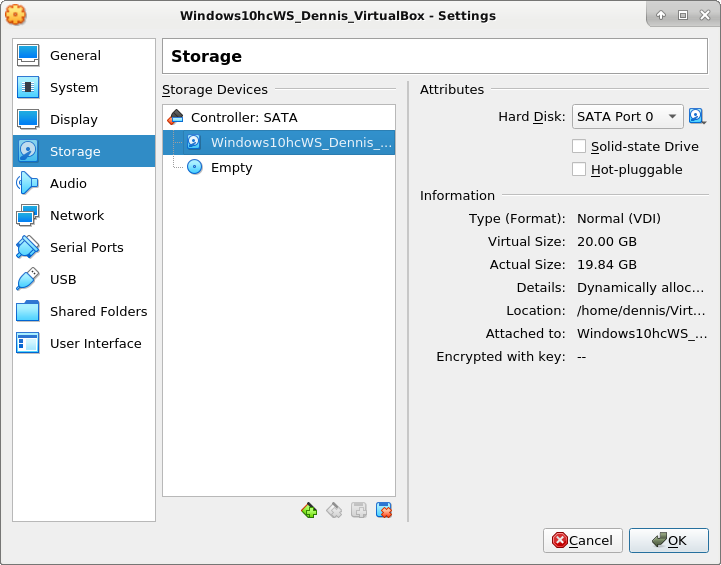
\includegraphics{virtualbox_settings_storage.png}
	\caption{VirtualBox New VM}
	\label{VB_settings_storage}
\end{figure}

Als je het CD-icoontje aanklikt krijg je een menu zoals weergegeven in figuur \ref{VB_settings_storage_cd_add}. Je ziet hier de ISO-images die je eerder gebruikt hebt en je kan ook een nieuwe ISO-image kiezen van af de harddisk.
\begin{figure}[H]
	\centering
	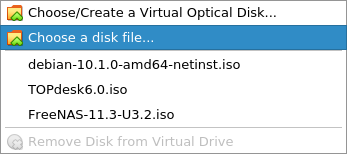
\includegraphics{virtualbox_settings_storage_cd_add.png}
	\caption{VirtualBox New VM}
	\label{VB_settings_storage_cd_add}
\end{figure}

Zodra je je bootable CD-image hebt toegevoegd aan de drive en in de boot order hebt aangegeven dat de CD voor de harddisk geprobeerd wordt, dan zal je systeem opstarten vanaf de (installatie) CD.

